\documentclass{article}[a4paper, 12pt]
\usepackage{minted}
\usepackage{csquotes}
\usepackage{french}
\usepackage{hyperref}
\usepackage[top=2.54cm, bottom=2.54cm, left=2.54cm, right=2.54cm]{geometry}
\usepackage[T1]{fontenc}
\usepackage{graphicx}
\bibliographystyle{alpha} %format des citations

\title{\LARGE \textbf{Cahier d’analyse des besoins } \\ \Large \textbf{Desert Fox}}
\author{Kristo Dhima, Garion Goubard,Sylvain Lascostes, \\Romain Réau, Vincent Samson et Alexandros Stergiou }
\date{Année universitaire 2021-2022}

\begin{document}
\maketitle

\tableofcontents %table des matière

\newpage

\section{Description du projet}

Le but de ce projet est de réaliser le moteur du jeu de guerre \emph{Desert Fox}. Le moteur contiendra une architecture qui puisse se déployer à travers Internet ou en local. L'interface graphique et les scénarios sera mis de côté afin de réaliser au mieux le moteur.\\

Deux joueurs vont devoir s'affronter sur une carte hexagonale. Le but du joueur de l'Axe est de sécuriser la Libye et l'Egypte en s'emparant d'Alexandrie, tandis que, le joueur Allié (Commonwealth et autres) protège Alexandrie et contenir les forces du joueur opposé.\\

Chaque tour de joueur possède plusieurs étapes:
\begin{itemize}
    \item Préparation
    \item Une suite d'actions ou les joueurs bougent leurs unités et les engagent au combat. Cette partie et divisée en 4 phases distinctes, ou le premier joueur alterne entre Allie et Axe a chaque fois:
    \begin{itemize}
        \item Mouvement du premier joueur
        \item Réaction du second joueur
        \item Combat du premier joueur.
    \end{itemize}
    \item Phase de réaménagement / reconstruction
\end{itemize}

La partie est hébergé sur un serveur afin de centraliser les données de la partie et simplifier les échanges client $\leftrightarrow$ serveur.

\section{Analyse de l'existant}

Divers projets open-source proposent des moteurs de jeu \emph{wargame}. Cependant la plupart de ces projets ne sont pas maintenu depuis plusieurs années ou elles ne sont pas adapté pour nos besoins. Comme la diversité des règles et d'extensions de \emph{Desert Fox}, qui ne peuvent pas être adapter aux moteurs de jeu existants.

\begin{itemize}
    \item Jeu Kriegsspiel : jeu de pions complexe développé par l'armée du royaume de Prusse au XIXe siècle pour enseigner les tactiques de combat aux officiers, adapte aussi dans des versions plus modernes \cite{livermore1879american}\\
   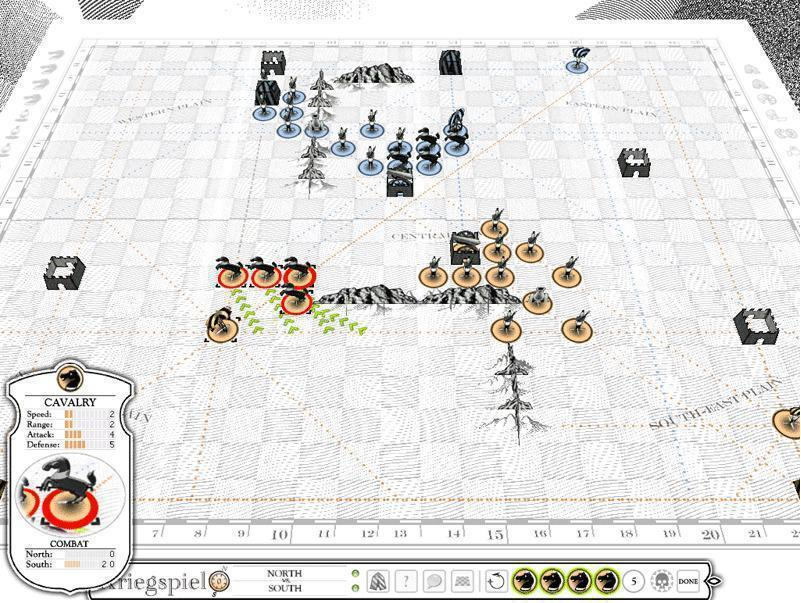
\includegraphics[scale=0.5]{kriegspiel.jpeg}
    
    
\end{itemize}


\section{Descriptions des besoins}
\subsection{Besoins Fonctionnels}
\subsubsection{Plateau de Jeu}

\begin{itemize}
    \item Définir la carte du jeu:
    \begin{itemize}
        \item Priorité 3/3, Les hexagones numérotés, chacun représentant une distance définie, par défaut : 16 kilomètres.
        \item Priorité 2/3, Différencier plusieurs types de terrain, les montages, les mers de sable et les crêtes par exemple.
        \item Priorité 1/3, Ajouter les différents types d'indicateurs afin d'illustrer les villages, les villes et les oasis par exemple.
    \end{itemize}
    \item Priorité 3/3, Définir les joueurs et leurs spécificités. Par exemple les nationalités possibles, le joueur qui joue le premier et celui qui a l'initiative.
    \item Priorité 3/3, Pouvoir poser des unités sur la carte et a retenir celles qui ne sont pas présentes dans celles-ci.
    \item Priorité 3/3, Pouvoir poser plusieurs unités sur un hexagone.
    \item Priorité 2/3, Pouvoir charger la carte du jeu à partir d'un fichier txt ou json et pouvoir la sauvegarder aux mêmes formats également.
    \item Priorité 3/3, Être capable de faire des lancés de dés et d'appliquer des modificateurs. La majeure partie du jeu se base sur les dés.
    \item Priorité 3/3, Définir une séquence de tour:
    \begin{itemize}
        \item Pouvoir alterner entre les joueurs.
        \item Respecter l'ordre strict d'un tour.
    \end{itemize}
    \item Priorité 2/3, Créer une base pour les cartes d'évènements. Celles-ci étant très différentes, l'implémentation sera limitée aux évènements génériques (non-spécifiques aux scénarios).
    \item Priorité 3/3, Pouvoir déterminer quel joueur a l'initiative.
    
\end{itemize}


\subsubsection{API}
\begin{itemize}
    \item Priorité 3/3, Pouvoir échanger des informations basiques entre serveur et client.
    \item Priorité 3/3, Pouvoir convertir un état de la carte du jeu en format utilisable par le client pour pouvoir ensuite afficher le plateau.
    \item Priorité 3/3, Envoyer un coup joue dans un format utile pour le serveur, pour pouvoir faire des éventuelles modifications sur le plateau.
    \item Priorité 3/3, Vérification des coups:
    \begin{itemize}
        \item Envoyer le coup joue au serveur.
        \item Vérifier que le coup est valide.
        \item Retourner une réponse positive ou négative. Si le coup est bon alors envoyer le nouvel état de le carte du jeu au client.
    \end{itemize}
    
\end{itemize}



\subsubsection{Unités}
\begin{itemize}
    \item Priorité 3/3, Définir l'unité comme entité abstraite, qui aura un morale, peut être perturbée (disrupted) et qui peut prendre des actions basiques comme attaquer et bouger.
    \item Priorité 3/3, Implémenter le système similaire à des points de vie (voir partie Depletion des règles).
    \item Priorité 2/3, Permettre aux unités éligibles de s'entraîner et de faire des upgrade.
    \item Priorité 3/3, Séparer les unités en catégories différentes: motorisées, à pied, mécanisées, cavalerie etc.
    \item Priorité 3/3, Mettre en place les situations ou l'unité devient perturbée:
    \begin{itemize}
        \item Trop de troupes sur un hexagone.
        \item Fin d'un mouvement de nuit.
        \item Après la phase de \"Supply Attrition\", il y a un échec sur le test d'usure (attrition).
    \end{itemize}
    \item Priorité 3/3, Créer un système de zones de contrôle (ZDC):
    \begin{itemize}
        \item Pouvoir calculer si une unité peut exercer une ZDC.
        \item Choisir quels hexagone sont dans cette ZDC.
        \item Appliquer des effets potentiels sur des unités présentes dans la ZDC.
        \item Permettre à certaines unités doivent ignorer les ZDC dans certaines phases d'un tour.
    \end{itemize}
    
\end{itemize}


\subsubsection{Organisation de l'armée}



\subsubsection{Mouvement}
\begin{itemize}
    \item Priorité 3/3, Le joueur du Commonwealth peut accélérer le mouvement de ses unités en utilisant le rail et transport maritime.
    L'utilisateur 
    \item Priorité 3/3, Mouvement la nuit.
\end{itemize}


\subsubsection{Combat}
\begin{itemize}
    \item Priorité 3/3 Pouvoir définir les unités participant au combat de ce round.
    \item Priorité 3/3 Pouvoir déterminer la puissance de combat de l'armée composée de ces unités.
    \item Priorité 3/3 Définir les règles du combat, par exemple le fait que seul les unités/armées adjacentes peuvent entrer en combat,par la volonté de l'attaquant.
    \item Priorité 1/3 Si un Hex contient plusieurs terrains, le défendant doit pouvoir en choisir un pour sa défense.
    \item Priorité 3/3 Pouvoir simuler le combat et donner les résultats.
    \item Priorité 3/3 Pouvoir simuler la retraite d'une armée si les spécifications le permettent, par exemple le terrain et la condition de l'armée est convenable, et si l'utilisateur le souhaite.
\end{itemize}


\subsubsection{Opérations Aériennes et Navales}
    \begin{itemize}
        \item Priorité 3/3 Pouvoir déterminer les différentes unités aériennes et navales ainsi que leurs spécificités.
        \item Priorité 3/3 Pouvoir déterminer les différentes cibles, comme par exemple des bases militaires ou les rivages(pour les opérations navales surtout), qu'ils peuvent cibler et attaquer.
        \item Priorité 3/3 En ce qui concerne les opérations navales, ils peuvent effectuer des expéditions transportant des munitions ainsi que des unités/machines de guerre.
    \end{itemize}



\subsubsection{Affichage}
\begin{itemize}
    \item Priorité 3/3, Afficher le joueur dont c'est le tour.
    \item Priorité 3/3, Déterminer et afficher les informations de fin de partie et du vainqueur.
    \item Priorité 3/3, Afficher les différents marqueurs sur l'état de chaque composante du jeu, par exemple hors d'approvisionnement pour les unités.
    \item Afficher le résultat et les informations a la fin du combat.
\end{itemize}


\subsection{Besoins Non-Fonctionnels}

\subsubsection{Affichage}
\begin{itemize}
    \item Affiche un message d'erreur ou de refus.
\end{itemize}

\subsubsection{Système}
\begin{itemize}
    \item Le temps d'attente entre un coup proposé et sa validité évalué devra être de l'ordre de la seconde.
\end{itemize}

\section{Justification/ Scénario}



\section{Tests et exemple}


\section{Bibliographie}
\bibliography{bibiography}

\end{document}